The bubble segmentation pipeline systematically processes raw manga pages---whether single-page or two-page spreads---through three sequential stages to extract individual speech bubble regions suitable for OCR processing, as illustrated in Figure \ref{fig:bubble-seg-pipeline}.

\begin{figure}[H]
    \centering
    \makebox[\textwidth][c]{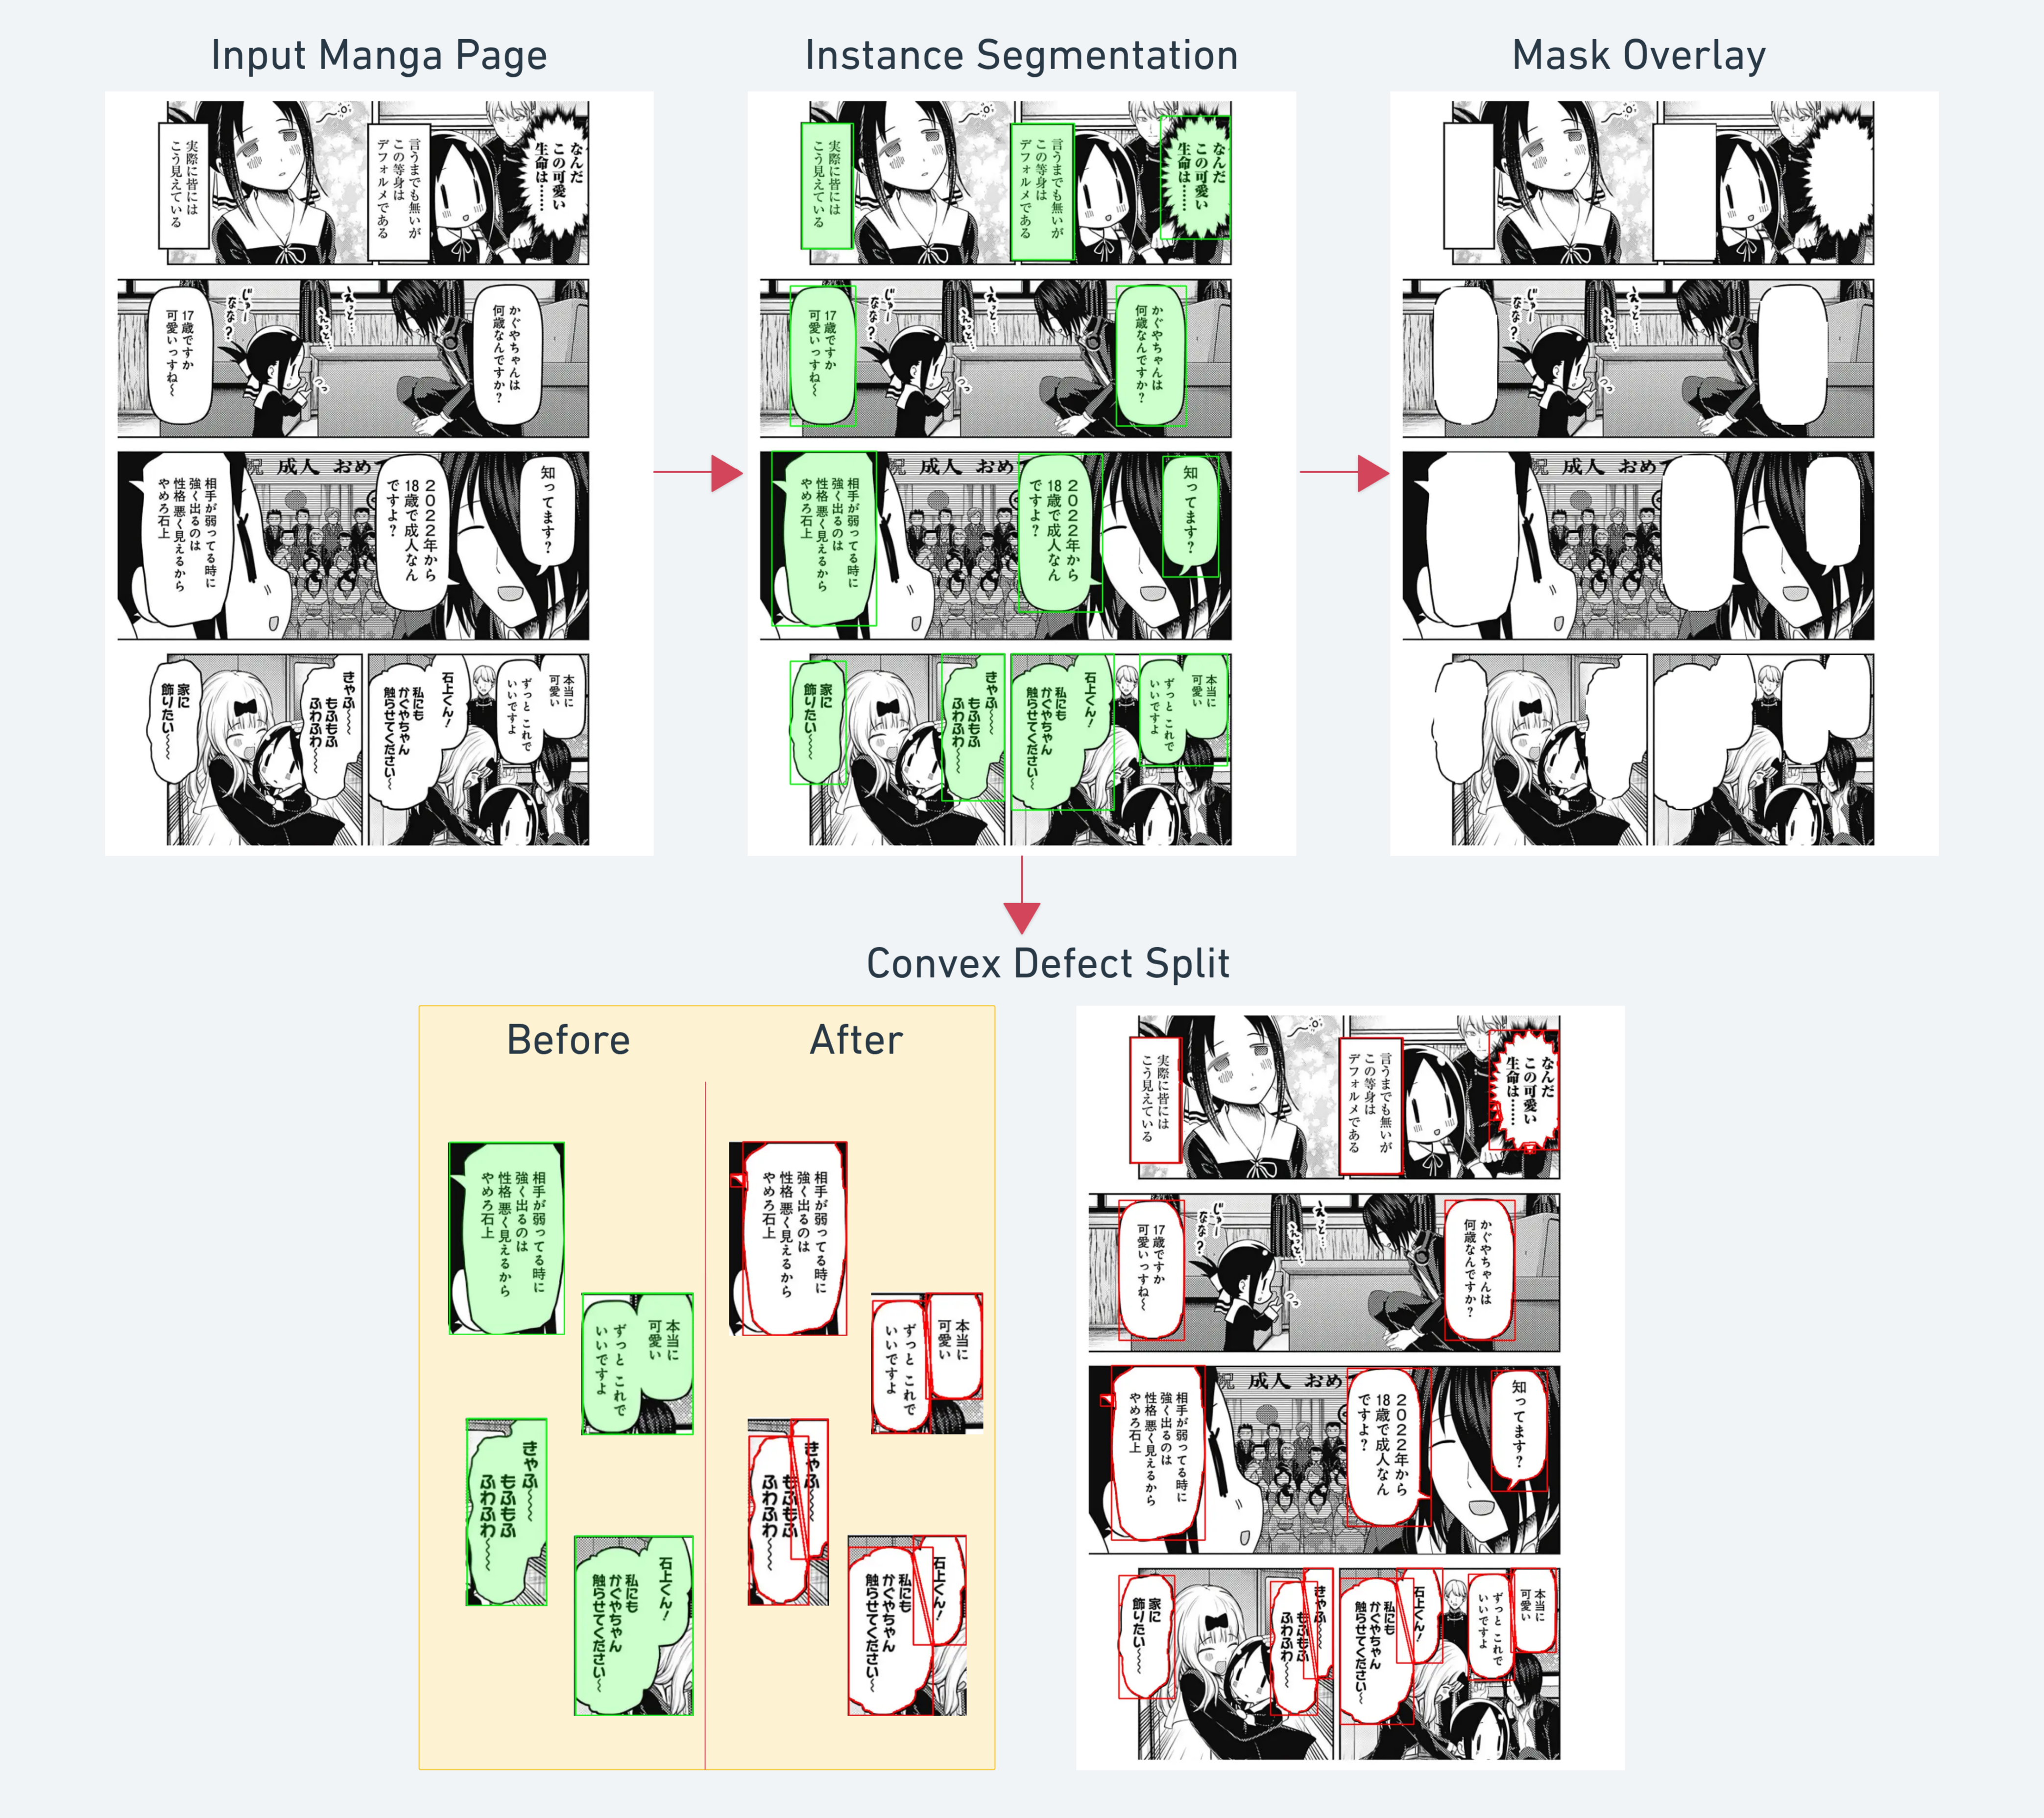
\includegraphics[width=1.5\textwidth]{img/segmentation_pipeline.pdf}}
    \caption{Bubble Segmentation Pipeline}
    \label{fig:bubble-seg-pipeline}
\end{figure}


The input manga page is processed through the YOLOv8 instance segmentation model, which generates pixel-precise segmentation masks for each detected speech bubble. These masks are visualized as green overlays in the figure, delineating the spatial extent of individual bubble regions across the page.\\

A critical step in the pipeline is overlaying the segmentation masks onto the original manga page to systematically erase all Japanese characters within the detected bubble regions. This mask-based whitening operation serves as an essential preparatory step for subsequent text replacement, ensuring clean canvas areas for the insertion of translated text.\\

While YOLO performs robust segmentation for isolated speech bubbles, it exhibits a fundamental limitation: when multiple bubbles are physically adjacent or overlapping, the model generates a single merged mask encompassing all connected regions. To address this deficiency, we implement a post-processing algorithm that analyzes convexity defects to identify merge boundaries and recursively splits connected bubble masks into discrete components. This splitting mechanism ensures that each speech bubble is processed independently during OCR, thereby maintaining text recognition accuracy.